\documentclass{eceasst}
% This is an empty ECEASST article that can be used as a template
% by authors.
% Just uncomment the appropriate frontmatter commands and provide
% the parameters.

% Required packages
% =================
\usepackage{multirow}
\usepackage{stmaryrd}
\usepackage{euscript}
\usepackage{amsmath}
\usepackage{textcmds}
\usepackage{wasysym}


\graphicspath{{images/}}


% Volume frontmatter
% ==================
% Volume frontmatter for GraBaTs 2014
% =====================================
\volume{X}{2014} % Volume number and year
\volumetitle{% Title of the volume (optional)
Proceedings of the\\
8th International Workshop on Graph-Based Tools\\
(GraBaTs 2014)}
\volumeshort{% Short title of the volume (optional)
Proc.\ GraBaTs 2014}
\guesteds{% Multiple guest editors
Matthias Tichy, Bernhard Westfechtel}


% Article frontmatter
% ===================
\title{Algebraic Specification to Realize the Diagram Predicate Framework} % Title of the article
\short{Algebraic Specification to Realize the Diagram Predicate Framework} % Short title of the article (optional)
%\author{\autref{1}\sponsor{}} % Authors and references to addresses
%\institute{\autlabel{1}} % Institutes with labels
%\abstract{} 
\keywords{model driven engineering, model transformation, metamodelling, rewriting theory, workflow model}

\begin{document}
\maketitle

% Main part of your article
% =========================
\section{Introduction}
Diagram Predicate Framework (DPF) provides a formal diagrammatic approach to metamodelling based on category theory and model transformation~\cite{Rutle10}. 
In this approach models at any level are formalised as diagrammatic specifications which consist of underlying graphs and diagrammatic constraints. 
The graphs represent the structures of the models; the diagrammatic constaints (also known as predicate constraints) are added to the structure; 
the graphs and constraints together provide the modelling formalisms of DPF. 
A DPF metamodelling hierarchy consists of metamodels, models and instances of models. 
A metamodel specification gives us a modelling language, the specification of a model represents a software system and the instances of models represent possible states of a software system. 
DPF has been extended in ~\cite{RutleMacCaullEtAl2012ECMFA,RutleWMFHIES12} for behavioural modelling. 
A workflow modelling language called DERF was developed and afterwords it was extended in \cite{WangRutleEtAl2012TASE} to define (static) semantics for timed and compensable workflow models and 
defined the dynamic semantics of models by a transition system where the states are instances and transitions are applications of transformation rules. 
An important observation of software systems is that very often they have different aspects such as user access, process flow, notification systems. 
In \cite{PAHI14} we introduced the use of multiple metamodelling for designing different aspects of systems that facilitates us with abstraction and less coupling among models. 

In this paper we provide the detailed semantics of multiple metamodelling with a running example from the healthcare domain. 
The DERF workflow language is not data aware and therefore it is not possible to specify actual business logics for tasks (also known as process) 
such as specifing \textit{preconditions} and/or \textit{postconditions}. In some other literature, \textit{Preconditions} and \textit{postconditions} are called branching conditions and 
task/process specification respectively.
In this article we present a new type of DPF construct named \textit{rewriting predicate} that permits us to specify model transformation rules in order to derive inferred knowledge or execute 
\textit{preconditions} and/or \textit{postconditions} for tasks. 
We present a graphical way of specifying \textit{preconditions} and \textit{postconditions} for tasks integrating DERF process model and Entity model. 
A DERF workflow model provides an abstraction of process flow, an entity model provides the data structure structure, and an integrated model provides us the details of a data aware workflow model
with graphically represented \textit{preconditions} and \textit{postconditions}. 
\textit{Rewriting predicates} also allows us to partially specify a model and derive a complete model by applying model transformation rules. 
This reduces the efforts required to explicitly specify the complete model of a system. 
So while designing a software model with DPF, a designer gets different abstraction level, perspective from different granularity to understand, and flexibility to modify the specification of a system. 

We used algebraic specification to realize the static and dynamic semantics of DPF specifications and the integration of multiple metamodels in this article. 
Although other executable systems may be used, to simulate the software model designed in DPF we propose the use of Maude system \cite{Bruni2006,Clavel2007} 
which is a high--level programming/specification/modeling language based on rewriting logic theory. 

In short, our main contribution in this article is as follows: 1) Extension of DPF with \textit{rewriting predicates}; 2) Integration of several metamodels; 3) Representation of DPF models in Maude. 
The paper is organized as follows: in section \ref{lbl:rewritingpredicate} we present \textit{rewriting predicate}, in section \ref{lbl:integration} we formally represent the integration of 
multiple metamodels, in section \ref{lbl:algebra} we provide the algebraic specification for DPF specifications, we present some related works in section \ref{lbl:relatedwork}, and 
in section \ref{lbl:conclusion} we conclude the paper with some future directions. 

\section{Rewriting Predicate}\label{lbl:rewritingpredicate}
A diagrammatic specification is formally specified in ~\cite{Rutle10} as a tuple $\mathfrak{S}$ $= (S, C^\mathfrak{S}:\Sigma)$ consisting of an underlying graph $S$ together with a set of 
$atomic$ $constraints$ $C^\mathfrak{S}$. The predicate constraints are from a predifined \textit{diagrammatic predicate signature} $\Sigma$ and they are used to add constraints to $S$. 
We modify the definition of \textbf{Signature} from ~\cite{Rutle10} with Definition.~\ref{def:Signature} in order to incorporate \textit{rewriting predicate} into $\Sigma$.


\begin{definition}[Signature]\label{def:Signature}
 A (diagrammatic predicate) signature $\Sigma$ = $(P^\Sigma, \alpha^\Sigma, \pi^\Sigma)$ consists of a collection of predicate symbols $P^\Sigma$ with two 
 multi-maps $\alpha^\Sigma, \pi^\Sigma$. The map $\alpha^\Sigma$ assigns graphs to predicate symbols $p \in P^\Sigma$ and $\alpha^\Sigma(p)$ is called the arity of the predicate symbol $p$. 
 The map $\pi^\Sigma$ assigns transformation rules to predicate symbols $p \in P^\Sigma$ and $\pi^\Sigma(p)$ is called the rewriting predicate of the predicate symbol $p$. 
\end{definition}

\begin{remark}
A predicate $p \in P^\Sigma$ is either a \textit{predicate constraint} (denoted as $dom(\alpha^\Sigma)$), iff $\alpha^\Sigma(p) \neq \phi$ 
or a \textit{rewriting predicate} (denoted as $dom(\pi^\Sigma)$) iff $\pi^\Sigma(p) \neq \phi$. 
\end{remark}



\begin{table}[h]\label{tbl:predicateconstraint}
 \caption{Predicate constraints of a sample signature $\Sigma_2$}
 \small
 \begin{center}
    \begin{tabular}{| l | c | c | p{6cm} | }    
    \hline
    $p$ & $\alpha^{\Sigma_2}(p)$ & Proposed Vis. & Semantic Interpretation \\ \hline
    [mult(n,m)] & 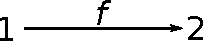
\includegraphics[width=0.13\textwidth]{mult.pdf} & 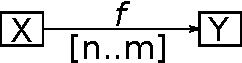
\includegraphics[width=0.16\textwidth]{mult_vis.pdf} & $\forall x \in X : m \leq |f(x)| \leq n$, 
																		  with $0 \leq m \leq n$ and $n \geq 1$ \\ \hline
    [irreflexive] & 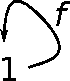
\includegraphics[width=0.05\textwidth]{irr_arity.pdf} & 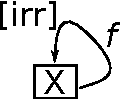
\includegraphics[width=0.09\textwidth]{irr_vis.pdf} & $\forall x \in X : x \notin f(x)$ \\ \hline
    [injective] & 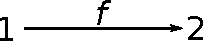
\includegraphics[width=0.13\textwidth]{mult.pdf} & 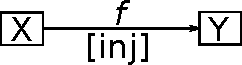
\includegraphics[width=0.16\textwidth]{inj_vis.pdf} & $\forall x,x' \in X :$ $f(x) = f(x')$ implies $x = x'$ \\ \hline
    [surjective] & 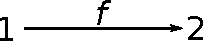
\includegraphics[width=0.13\textwidth]{mult.pdf} & 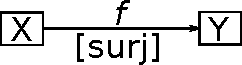
\includegraphics[width=0.16\textwidth]{surj_vis.pdf} & $\forall y \in Y, \exists x \in X, f(x) = y $ \\ \hline
    %\multirow{1}{*}{[inverse]} & \multirow{1}{*}{ 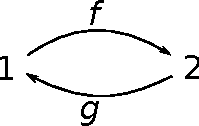
\includegraphics[width=0.16\textwidth]{inv_1.pdf}} & \multirow{1}{*}{ 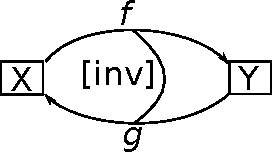
\includegraphics[width=0.16\textwidth]{inv_vis.pdf}} & \multirow{1}{*}{ $\forall x \in X, \forall y \in Y :$  $y \in f(x)$ iff $x \in g(y) $ } \\
    [inverse] & 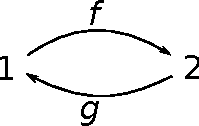
\includegraphics[width=0.13\textwidth]{inv_1.pdf} & 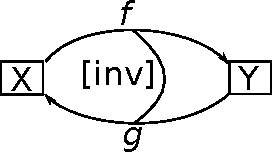
\includegraphics[width=0.16\textwidth]{inv_vis.pdf} & $\forall x \in X, \forall y \in Y :$  $y \in f(x)$ iff $x \in g(y) $  \\ \hline 
    [image-inclusion] & 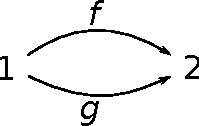
\includegraphics[width=0.13\textwidth]{img_1.pdf} & 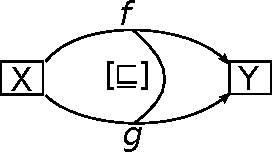
\includegraphics[width=0.16\textwidth]{img_vis.pdf} & $\forall x \in X :$  $f(x) \subseteq g(x) $  \\     
    \hline    
    \end{tabular}
    \end{center}
\end{table}
\normalsize






Table.~\ref{tbl:predicateconstraint},~\ref{tbl:rewritingpredicate} shows a sample signature $\Sigma_2 = (P^{\Sigma_2}, \alpha^{\Sigma_2}, \pi^{\Sigma_2})$ where the first column of 
both tables show the names of the predicates; the second, third and fourth columns of Table.~\ref{tbl:predicateconstraint} show the arities of predicates, a possible visualization 
and the semantic interpretation respectively; the second and third columns of Table.~\ref{tbl:rewritingpredicate} show the transformation rules of predicates and a possible visualization respectively.
For readability reasons, the semantic interpretations of \textit{predicate constraints} are presented in a set--theoretical indexed manner in Table.~\ref{tbl:predicateconstraint}, 
although the actual semantics of each predicate constraint $p \in P^{\Sigma}$ of a sample signature $\Sigma$ is defined in \cite{Rutle10} by a set $\llbracket p \rrbracket^{\Sigma}$ of 
graph homomorphisms $\iota : O \rightarrow \alpha^{\Sigma}(p)$ called valid instances of $p$, where $O$ may vary over all graphs. 
For example, the valid instances of $[inverse]$ \textit{predicate constraint} of signature $\Sigma_2$ (see Table.~\ref{tbl:predicateconstraint}) are defined as follows. 
%In this situation, $\llbracket inverse \rrbracket^{\Sigma_2} = \{ \iota_1, \iota_2, \iota_3, \iota_4, \iota_5 \}$ is a set of graph homomorphisms that provides the semantics of $[inverse]$. 
All valid instances of $\llbracket inverse \rrbracket^{\Sigma_2}$ that provides the semantics of $[inverse]$ are provided below: 



\begin{center}
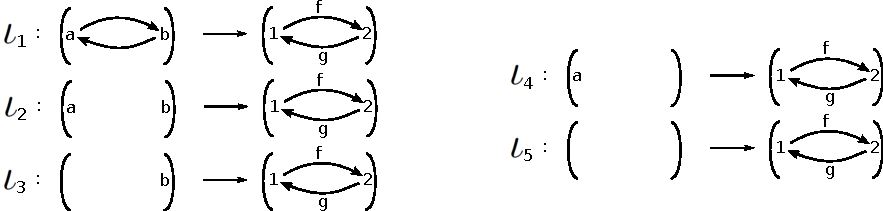
\includegraphics[width=0.7\textwidth]{inv-hom-set.pdf}
\end{center}

On the other hand, the semantics of \textit{rewriting predicates} are defined by coupled transformation \cite{SLK11} rules with negative application conditions as in Table.~\ref{tbl:rewritingpredicate}. 


\begin{table}[h]\label{tbl:rewritingpredicate}    
 \caption{Rewriting predicates of a sample signature $\Sigma_2$}
 \small
 \begin{center}
    \begin{tabular}{| l | c | c | c | }    
    \hline
    \multirow{2}{*}{$p$} & \multicolumn{2}{c |}{$\pi^{\Sigma_2}(p)$} & \multirow{2}{*}{Proposed Vis.} \\ \cline{2-3}
        & $(\mathfrak{N}_0 \rightarrow \mathfrak{N}_{1})$ $\xleftarrow{\makebox[1cm]  n  }$  $(\mathfrak{L}_0 \rightarrow \mathfrak{L}_{1}) $ & $(\mathfrak{R}_0 \rightarrow \mathfrak{R}_{1}) $ &   \\ \hline    
    \multirow{2}{*}{[opposite]} 		& 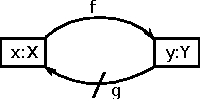
\includegraphics[width=0.13\textwidth]{inv-1.pdf} & 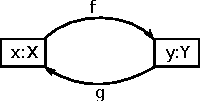
\includegraphics[width=0.13\textwidth]{inv-R.pdf} & \multirow{2}{*}{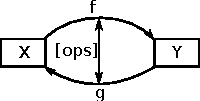
\includegraphics[width=0.13\textwidth]{inv-vis.pdf}}  \\ \cline{2-3}
			& 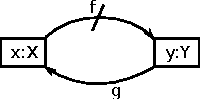
\includegraphics[width=0.13\textwidth]{inv-2.pdf} & 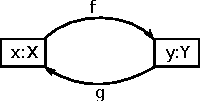
\includegraphics[width=0.13\textwidth]{inv-R.pdf} &  \\ \hline
    [composition] 	& 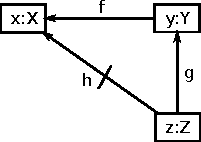
\includegraphics[width=0.13\textwidth]{comp-L.pdf} & 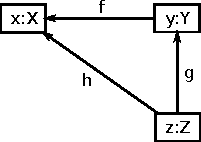
\includegraphics[width=0.13\textwidth]{comp-R.pdf} & 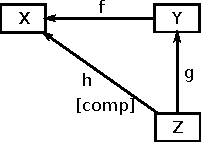
\includegraphics[width=0.13\textwidth]{comp-vis.pdf}  \\ \hline 			
    [inheritance] 	& 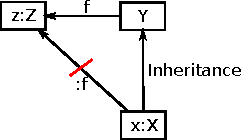
\includegraphics[width=0.09\textwidth]{inheritance-L.pdf} & 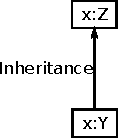
\includegraphics[width=0.09\textwidth]{inheritance-R.pdf} & 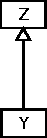
\includegraphics[width=0.03\textwidth]{inheritance-vis.pdf}  \\ 
    \hline    
    \end{tabular}
    \end{center}
\end{table}
\normalsize

\begin{definition}[Semantics of Rewriting Predicates]
 The semantics of a rewriting predicate $p \in P^{\Sigma_{i+1}}$ is given by a set of coupled transformation rules where each transformation 
 rule $r: (\mathfrak{L}_i \rightarrow \mathfrak{L}_{i+1})   \leftarrow (\mathfrak{K}_i \rightarrow \mathfrak{K}_{i+1})  \rightarrow 
 (\mathfrak{R}_i \rightarrow \mathfrak{R}_{i+1}) $ has a negative application condition and there exists a specification morphism 
 $n: (\mathfrak{L}_i \rightarrow \mathfrak{L}_{i+1}) \rightarrow (\mathfrak{N}_i \rightarrow \mathfrak{N}_{i+1}) $. 
\end{definition}

Notice that the matching patterns $(\mathfrak{L}_i \rightarrow \mathfrak{L}_{i+1})$ and negative application conditions $(\mathfrak{N}_i \rightarrow \mathfrak{N}_{i+1}) $ 
are represented in the same diagram in 
Table.~\ref{tbl:rewritingpredicate} to make it more readable. Negative application conditions are striked through in the diagram to represent that they must not exist while matching. 
Now it is worthwhile to make a comparison between these two types of predicates. 
\textit{Predicate constraints} do not derive any change to an instance of a specification whereas \textit{rewriting predicates} may change the strucutre of an instance. 
By defining \textit{predicate constraints} we can specify some structural constraints and can decide if an instance is a valid instance of a specification. 
In order to be consistent we need to modify the definition of \textbf{Atomic Constraint} and \textbf{Specification} from \cite{Rutle10} and include a new definition for \textbf{Rewriting Rule} as follows:


\begin{definition}[Atomic Constraint]
 Given a signature $\Sigma = (P^\Sigma, \alpha^\Sigma, \pi^\Sigma)$, an atomic constraint $(p, \delta)$ added to a graph $S$ is given by a predicate symbol $p$ and a graph 
 homomorphism $\delta : \alpha^{\Sigma}(p) \rightarrow S$ where $p \in P^\Sigma$ is a predicate. 
\end{definition}



\begin{definition}[Rewriting Rule]
 Given a signature $\Sigma = (P^\Sigma, \alpha^\Sigma, \pi^\Sigma)$, a rewriting rule $(r, \delta)$ attached to a graph $S$ is given by a predicate symbol $r$ and a graph 
 homomorphism $\delta : \pi^{\Sigma}(r) \rightarrow ((I, \iota) \rightarrow S)$ where $r \in P^\Sigma$ is a predicate. 
\end{definition}


\begin{definition}[Specification]
 Given a signature $\Sigma = (P^\Sigma, \alpha^\Sigma, \pi^\Sigma)$, a (diagrammatic) specification $\mathfrak{S} = (S, C^{\mathfrak{S}}:\Sigma, R^{\mathfrak{S}}:\Sigma )$ 
 is given by 
 a graph $S$, 
 a set $C^\mathfrak{S}$ of atomic constraints $(p, \delta)$ on $S$ with $p \in dom(\alpha^\Sigma)$, and
 a set $R^\mathfrak{S}$ of rewriting rules $(r, \delta)$ on $S$ with $r \in dom(\pi^\Sigma)$. 

\end{definition}



Lets take the following requirements of a healthcare domain to develop an entity diagram using DPF:


\textbf{1.} \textit{An employee (e.g., nurse, doctor) must work for a department. }

\textbf{2.} \textit{A department may have zero or more employees. }

\textbf{3.} \textit{An ward must be under a department. }

\textbf{4.} \textit{An employee who is involved in a ward, must work in the controlling department. }

\textbf{5.} \textit{Every person has a name. }

\textbf{6.} \textit{A person could be a Patient or an Employee. }

\textbf{7.} \textit{Patients systolic and diastolic blood pressure records are natural numbers. }






\begin{figure}[h]
\centering
 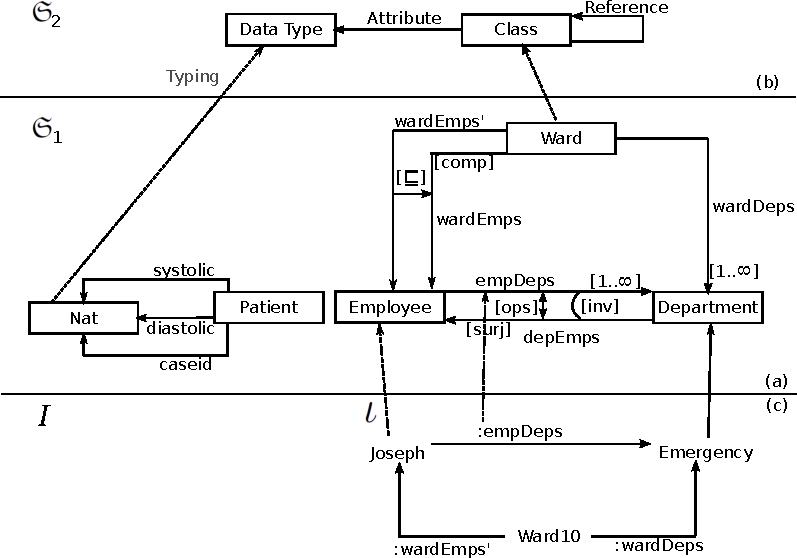
\includegraphics[width=0.65\textwidth]{entity-1.pdf}
 \caption{ a) Entity specification $\mathfrak{S}_1 = (S, C^{\mathfrak{S}_1} : \Sigma_2 , R^{\mathfrak{S}_1} : \Sigma_2)$, b) its meta model $\mathfrak{S}_2$, and c) an instance $(I,\iota)$ of $\mathfrak{S}_1$}
 \label{fig:entity-diagram}
 \end{figure}

Fig.~\ref{fig:entity-diagram}(a) shows an entity specification $\mathfrak{S}_1$ that we developed from the above mentioned requirements. 
In this specification we used the signature $\Sigma_2$ from Table.~\ref{tbl:predicateconstraint} and ~\ref{tbl:rewritingpredicate} to define the set $C^{\mathfrak{S}_1}$ of atomic constraints 
(see Table.~\ref{tbl:atomicconstraint}) and a set $R^{\mathfrak{S}_1}$ of \textit{rewriting rules} (see Table.~\ref{tbl:rewritingrules}). 
Requirement 1 is encoded in $\mathfrak{S}_1$ by the $[surjective]$ \textit{predicate constraint} over the morphism $depEmps$; 
the fourth requirement ``an employee who is involved in a ward, must work in the controlling department'' is encoded in $\mathfrak{S}_1$ by a \textit{rewriting predicate} $[composition]$ 
and a \textit{predicate constraint} $[image-inclusion]$ over morphisms $depEmps$, $wardDeps$, $wardEmps$ and $wardEmps'$ where $wardEmps$ := $wardDeps; depEmps$ 
(the composition of morphisms $wardDeps$ and $depEmps$).

\begin{figure}[t]
\centering
 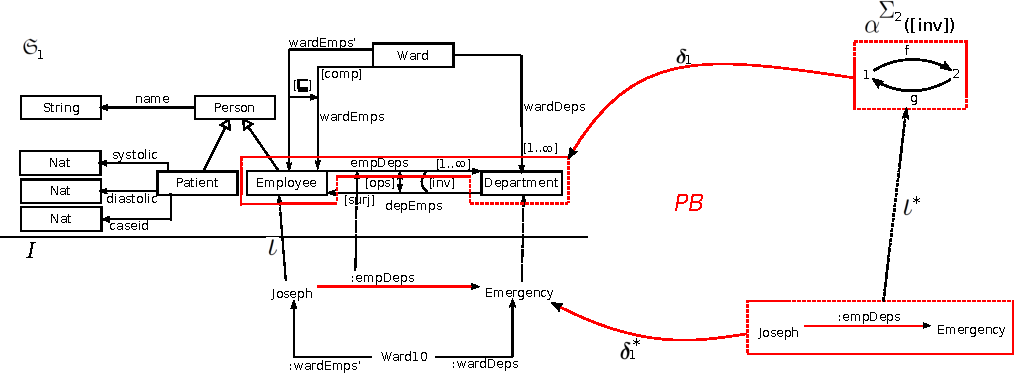
\includegraphics[width=0.9\textwidth]{entity-1-pullback.pdf}
 \caption{ Pullback $\alpha^{\Sigma_2}([inv]) \xleftarrow{\iota^*} O^* \xrightarrow{\delta_1^*} I $ of $\alpha^{\Sigma_2}([inv]) \xrightarrow{\delta_1} S \xleftarrow{\iota} I $ }
 \label{fig:entity-pb}
 \end{figure}
 

\begin{table}[h]\label{tbl:atomicconstraint}
 \caption{The set of atomic constraints $C^{\mathfrak{S}_1}$ of  $\mathfrak{S}_1$}
 \small
 \begin{center}
    \begin{tabular}{| l | c | c | }    
    \hline
    $(p,\delta)$ & $\alpha^{\Sigma_2}(p)$ & $\delta(\alpha^{\Sigma_2}(p))  $ \\ \hline
    $([mult(1,\infty)], \delta_1)$ & 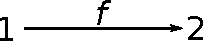
\includegraphics[width=0.13\textwidth]{mult.pdf} & 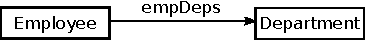
\includegraphics[width=0.3\textwidth]{atomic_delta1.pdf}  \\ \hline    
    $([mult(1,\infty)], \delta_2)$ & 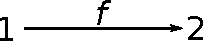
\includegraphics[width=0.13\textwidth]{mult.pdf} & 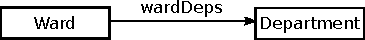
\includegraphics[width=0.3\textwidth]{atomic_delta2.pdf}  \\ \hline    
    $([surjective], \delta_3)$ & 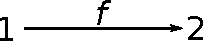
\includegraphics[width=0.13\textwidth]{mult.pdf} & 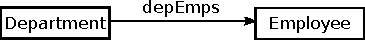
\includegraphics[width=0.3\textwidth]{atomic_delta3.pdf}  \\ \hline    
    $([inverse], \delta_4)$ & 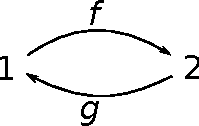
\includegraphics[width=0.11\textwidth]{inv_1.pdf} & 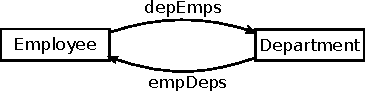
\includegraphics[width=0.3\textwidth]{atomic_delta4.pdf}  \\ \hline    
    $([image-inclusion], \delta_5)$ & 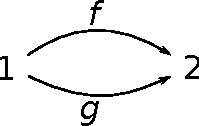
\includegraphics[width=0.11\textwidth]{img_1.pdf} & 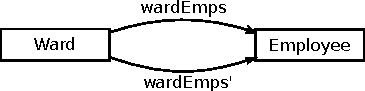
\includegraphics[width=0.3\textwidth]{atomic_delta5.pdf}  \\   
    \hline    
    \end{tabular}
    \end{center}
\end{table}
\normalsize

\begin{table}[h]\label{tbl:rewritingrules}    
 \caption{The set of rewriting rules $R^{\mathfrak{S}_1}$ of  $\mathfrak{S}_1$}
  \tiny
 \begin{center}
    \begin{tabular}{| l | c | c | c | c | }    
    \hline
    
    \multirow{2}{*}{$(r,\delta)$} & \multicolumn{2}{c |}{$\pi^{\Sigma_2}(r)$} & \multicolumn{2}{c |}{ $\delta(\pi^{\Sigma_2}(r))$ }\\ \cline{2-5}
        & $(\mathfrak{N}_0 \rightarrow \mathfrak{N}_{1})$ $\xleftarrow{\makebox[0.3cm]  n  }$  $(\mathfrak{L}_0 \rightarrow \mathfrak{L}_{1})$ & $(\mathfrak{R}_0 \rightarrow \mathfrak{R}_{1}) $ & 
			      $\delta(\mathfrak{N}_0 \rightarrow \mathfrak{N}_{1}) \xleftarrow{\makebox[0.3cm] n} \delta( \mathfrak{L}_0 \rightarrow \mathfrak{L}_{1})$  & $\delta(\mathfrak{R}_0 \rightarrow \mathfrak{R}_{1})$ \\ \hline    
    \multirow{2}{*}{$([opposite], \delta_6)$}  & 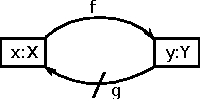
\includegraphics[width=0.13\textwidth]{inv-1.pdf} & 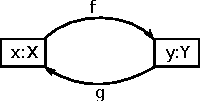
\includegraphics[width=0.13\textwidth]{inv-R.pdf} & 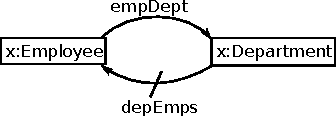
\includegraphics[width=0.19\textwidth]{inv-1-delta.pdf} & 
				    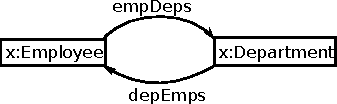
\includegraphics[width=0.19\textwidth]{inv-R-delta.pdf}  \\ \cline{2-5}
				  & 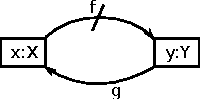
\includegraphics[width=0.13\textwidth]{inv-2.pdf} & 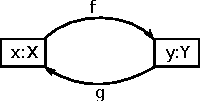
\includegraphics[width=0.13\textwidth]{inv-R.pdf} &  
				  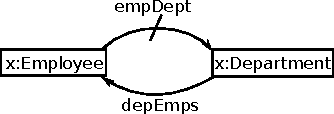
\includegraphics[width=0.19\textwidth]{inv-2-delta.pdf} & 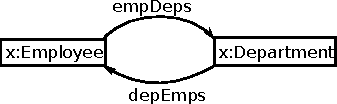
\includegraphics[width=0.19\textwidth]{inv-R-delta.pdf} \\ \hline    
    $([composition], \delta_7)$ 		  & 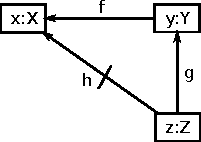
\includegraphics[width=0.13\textwidth]{comp-L.pdf} & 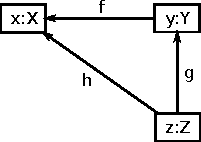
\includegraphics[width=0.13\textwidth]{comp-R.pdf} & 
				    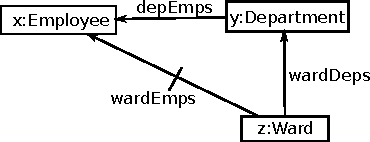
\includegraphics[width=0.19\textwidth]{comp-L-delta.pdf} & 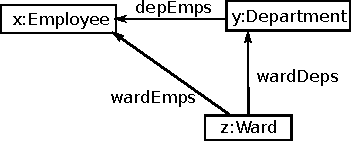
\includegraphics[width=0.19\textwidth]{comp-R-delta.pdf} \\ \hline 			
    $([inheritance], \delta_8)$ 		  & \includegraphics[width=0.08\textwidth]{inheritance-L.pdf} & \includegraphics[width=0.08\textwidth]{inheritance-R.pdf} & 
				    \includegraphics[width=0.10\textwidth]{inheritance-L-delta.pdf} & \includegraphics[width=0.10\textwidth]{inheritance-R-delta.pdf} \\ \hline
    $([inheritance], \delta_9)$ 		  & \includegraphics[width=0.08\textwidth]{inheritance-L.pdf} & \includegraphics[width=0.08\textwidth]{inheritance-R.pdf} & 
				    \includegraphics[width=0.10\textwidth]{inheritance2-L-delta.pdf} & \includegraphics[width=0.10\textwidth]{inheritance2-R-delta.pdf} \\ 				    
    \hline    
    \end{tabular}
    \end{center}
\end{table}
\normalsize



Fig.~\ref{fig:entity-diagram}(a) shows a possible instance $(I, \iota)$ of $\mathfrak{S}_1$. 
Even though $I$ is typed by $S$, it is not a valid instance of $\mathfrak{S}_1$ since it does not satisfy the \textit{predicate constraints} $[surjective]$, $[inverse]$ and $[image-inclusion]$. 
We explain this by a pullback operation in Fig.~\ref{fig:entity-pb}. Since $\iota^* \notin \llbracket inverse \rrbracket^{\Sigma_2}$, $I$ does not satisfy $[inverse]$. 
Similarly we can explain why $I$ does not satisfy $[surjective]$ and $[image-inclusion]$. 



 
Until at this point we have not considered the execution of \textit{rewriting rules} over $(I, \iota)$. 
By applying \textit{rewriting rules} from Table.~\ref{tbl:rewritingrules} over $(I, \iota)$ we may derive new information. 
An instance of a specification where \textit{rewriting rules} are applicable is called a partial instance. 
The \textit{rewriting predicate} $[opposite]$ is used to derive morphism $y \xrightarrow{g} x$ (if it does not exist) from the existance of a morphism $x \xrightarrow{f} y$ or vice versa; 
$[composition]$ is used to derive morphism $z \xrightarrow{h} x$ (if it does not exist) from the existance of morphisms $z \xrightarrow{g} y$ and $y \xrightarrow{f} x$; 
$[inheritance]$ derives a typing morphism $x \rightarrow Z$ (if it is not present) if $x \rightarrow Y$ and $Z$ is a superclass of $Y$. 
Once we apply the \textit{rewriting rules} for $[opposite]$, $[composition]$ and $[inheritance]$ over $(I, \iota)$ we get a complete instance of specification $\mathfrak{S}_1$ as shown in 
Fig.~\ref{fig:entity-1-full}. We call it a complete instance of $\mathfrak{S}_1$ as no more \textit{rewriting predicates} are further applicable on $(I, \iota)$. 
This complete instance is a valid instance of $\mathfrak{S}_1$ as it satisfies all atomic constraints. 
Now it is easy to understand the motivation of using \textit{rewriting predicates} in DPF as it permits us to specify partial instance of a specification. 
We may utilize the reasoning capability of \textit{rewriting predicates} to derive a complete instance from a partially specified instance. 



\begin{figure}[h]
\centering
 \includegraphics[width=0.65\textwidth]{entity-1-full.pdf}
 \caption{ a) Entity specification $\mathfrak{S}_1 = (S, C^{\mathfrak{S}_1} : \Sigma_2,  R^{\mathfrak{S}_1} : \Sigma_2)$ and  b) a complete instance $(I, \iota)$ of $\mathfrak{S}_1$}
 \label{fig:entity-1-full}
 \end{figure}





\begin{definition}[Application of Rewriting Rules]
 Let $(\Sigma_1 \rhd S_1, \mathfrak{S}_1, \Sigma_2)$ be a modelling formalism where specification $\mathfrak{S}_1 = (S_1, C^{\mathfrak{S}_1}:\Sigma_2, R^{\mathfrak{S}_1}:\Sigma_2)$ 
 has a set $R^{\mathfrak{S}_1}$ of rewriting rules $(r, \delta)$ on $S_1$.
 Each rewriting rule $(r, \delta)$ is associated with a set of coupled transformation rules $\pi^{\Sigma_2}(r)$. 
Each transformation rule $t \in \pi^{\Sigma_2}(r)$ has a negative application condition. 
A rule $t: (\mathfrak{L}_0 \rightarrow \mathfrak{L}_1) \leftarrow (\mathfrak{K}_0 \rightarrow \mathfrak{K}_1) \rightarrow  (\mathfrak{R}_0 \rightarrow \mathfrak{R}_1)$ 
is applicable over $\mathfrak{S}_0 \rhd S_1$ 
if there is a match $m : \delta( \mathfrak{L}_0 \rightarrow \mathfrak{L}_1) \rightarrow (\mathfrak{S}_0 \rightarrow \mathfrak{S}_1)$ 
and there does not exist any match to the negative application condition, $q : \delta( \mathfrak{N}_0 \rightarrow \mathfrak{N}_1) \rightarrow (\mathfrak{S}_0 \rightarrow \mathfrak{S}_1)$ 
such that $m = n ; q$. 

\begin{center}
\includegraphics[width=0.5\textwidth]{dpo.pdf}
\end{center}
\end{definition}


\begin{definition}[Partial and Complete Instance]
 Let $\mathfrak{S} = (S, C^{\mathfrak{S}}:\Sigma, R^{\mathfrak{S}}:\Sigma )$ be a specification with 
 a graph $S$, 
 a set $C^\mathfrak{S}$ of atomic constraints $(p, \delta)$ on $S$ with $p \in dom(\alpha^\Sigma)$, and
 a set $R^\mathfrak{S}$ of rewriting rules $(r, \delta)$ on $S$ with $r \in dom(\pi^\Sigma)$. 
 An instance $(I, \iota)$ is a \textit{partial instance} of $\mathfrak{S}$ if there exist some rewriting rules $(r, \delta) \in R^{\mathfrak{S}}$ those are applicable over $(I, \iota)$. 
 An instance $(I, \iota)$ is a \textit{complete instance} of $\mathfrak{S}$ if there does not exist any rewriting rule $(r, \delta) \in R^{\mathfrak{S}}$ that is applicable over $(I, \iota)$. 

\end{definition}


\begin{remark}
A complete instance $(I, \iota)$ is a valid instance of specification $\mathfrak{S}$ if it does not violate any constraint from $C^{\mathfrak{S}}$. We denote it as $(I, \iota) \RHD \mathfrak{S}$
\end{remark}


\section{Integration of Multiple Metamodels}\label{lbl:integration}
In this section we formally define the integration of specifications and provide its syntax and semantics with a running example. 

\begin{definition}[Integrated Specification]
 Given two complete and valid specifications $\mathfrak{S} = (S, C^{\mathfrak{S}}: \Sigma^S, R^{\mathfrak{S}}: \Sigma^S)$ and 
 $\mathfrak{T} = (T, C^{\mathfrak{T}}: \Sigma^T, R^{\mathfrak{T}}: \Sigma^T)$, 
 their integration $\mathfrak{J} = (J, C^{\mathfrak{J}}: \Sigma^J, R^{\mathfrak{J}}:\Sigma^J)$ is given 
 %by a graph $J = (S \uplus T)$: a disjoint union of the underlying graphs of $\mathfrak{S}$ and $\mathfrak{T}$, 
 %a set $C^{\mathfrak{J}}$ of atomic constraints $(p, \delta)$ on $J$ with $p \in dom(\alpha^{\Sigma^J})$ 
 a set $R^{\mathfrak{J}}$ of rewriting rules $(r,\delta)$ on $J$ with $r \in dom(\pi^{\Sigma^J})$ and
 by two inclusion specification morphisms $\phi^S : \mathfrak{S} \hookrightarrow \mathfrak{J}$, $\phi^T : \mathfrak{T} \hookrightarrow \mathfrak{J}$ 
 such that the following diagram commutes:
  
\begin{center}
\includegraphics[width=0.4\textwidth]{spec-morphism.pdf}
\end{center}  
 
\end{definition}

\begin{remark}
 The underlying graph $J = (S \uplus T)$ of the integrated specification $\mathfrak{J}$ is a disjoint union of the underlying graphs of $\mathfrak{S}$ and $\mathfrak{T}$. 
 The set $R^{\mathfrak{J}}$ of rewriting rules $(r,\delta)$ on $J$ is defined by a set of coupled transformation rules. 
\end{remark}

\begin{proposition}
 The integration of two complete and valid instances $(S_0, \iota^S), (T_0, \iota^T)$ of specifications $\mathfrak{S}$ and $\mathfrak{T}$ respectively is a partial instance 
 $(J_0, \iota^J)$ of $\mathfrak{J}$.  
\end{proposition}

The integrated partial instance $(J_0, \iota^J)$ is a typed specification $J_0 \rhd J$ that becomes a complete instance $J_0^*$ of the integrated specification 
$\mathfrak{J}$ by iterative applications of the set $R^{\mathfrak{J}}$ of rewriting rules. 
Applying pullback over a complete integrated specification $J_0^*$ we get two instances $(S_0', \iota^S)$ and $(T_0', \iota^T)$ of 
specifications $\mathfrak{S}$ and $\mathfrak{T}$ respectively.

\begin{center}
\includegraphics[width=0.25\textwidth]{intr-pb.pdf}
\end{center}

\noindent
$(S_0', \iota^S)$ and $(T_0', \iota^T)$ may be partial instances with respect to their specifications and further rewriting rules may be applicable 
from the set $R^{\mathfrak{S}}$ and $R^{\mathfrak{T}}$. The complete and valid instances $(S_0^*, \iota^S), (T_0^*, \iota^T)$ of $\mathfrak{S}$ and $\mathfrak{T}$ after applying rewriting rules, 
may be integrated again and be used for further derivation. This derivation process can run again and again until no further rewriting rule is applicable: 

\begin{center}
\includegraphics[width=0.35\textwidth]{fixpoint.pdf}
\end{center}

As an example for the integration of multiple metamodels we take a DERF process model and an entity model from a healthcare domain and present a data aware workflow model.
Fig.~\ref{fig:bp} shows a hypertension management workflow model with its meta model. The workflow model is developed from a clinical practice guideline \cite{HTN}. 


\begin{figure}[h]
\centering
 \includegraphics[width=\textwidth]{bp.pdf}
 \caption{Example DERF process model specification: Hypertension Workflow Model}
 \label{fig:bp}
 \end{figure}
 
The behavior of DERF process models are given by a coupled transition system. 
The hypertension workflow model consists of some predicates \textit{[XOR SPLIT]}, \textit{[AND SPLIT]}, \textit{[OR SPLIT]}, etc,. which describes the control flow of the process model. 
The dynamic semantics of DERF workflow models are provided in ~\cite{RutleMacCaullEtAl2012ECMFA}. 
The predicates \textit{[Disabled]}, \textit{[Enabled]}, etc,. from predicate signature $\Sigma_1^T$ are annotations and they do not have a semantic counterpart. 
Task instances with annotations in specification $\mathfrak{S}_0$ give us a state of a workflow instance. 
And the coupled transition systems produce reachable instances of a workflow model from an initial instance. 


Fig.~\ref{fig:bp-instance} shows two specifications $\mathfrak{T}_0$ and $\mathfrak{T}_0'$ which are reachable instances of $\mathfrak{T}_1$ . 
The predicate $[c,11]$ denotes that they are the instance of case no 11. For every patient there are different instances with different case numbers. 
In $\mathfrak{T}_0$ the task instance \textit{:Initial BP Measure} is finished (annotated with $<F>$), the branch \textit{:f} and \textit{:g} are evaluated to true and false recursively and both task instances 
\textit{:Safe} and \textit{:Visit1} are disabled (annotated with $<D>$). 
In $\mathfrak{T}_0′$ the task instance \textit{:Safe} is enabled (annotated with $<E>$).

\begin{figure}[h]
\centering
 \includegraphics[width=0.6\textwidth]{bp-instances.pdf}
 \caption{Two reachable instances of the hypertension workflow model}
 \label{fig:bp-instance}
 \end{figure}

We design a data aware process model specification $\mathfrak{J}_1$ by integrating the hypertension workflow model specification $\mathfrak{T}_1$ and 
the entity specification $\mathfrak{S}_1$ from Fig.~\ref{fig:entity-diagram}. 
For the integrated specification $\mathfrak{J}_1$ we need to specify a set of atomic constraints and a set of rewriting rules. 
We may use the predicate symbols associated with the shape graphs $S, T$ from $\Sigma_2^S, \Sigma_2^T$ and from the predicate signatures $\Sigma_1^S, \Sigma_1^T$ of specifications 
$\mathfrak{S}_1, \mathfrak{T}_1$. For this particular example, we defined a set $R^{\mathfrak{J}_1}$ of rewriting rules $(r, \delta)$ for the integrated specification. 
Table.~\ref{tbl:highbp} shows the transformation rule of predicate $[HighBP]$. 
In the transformation rule we included a \textit{condition} of the form $(\forall X) \varphi : \bigwedge_i$ $p_i = q_i$ where all the variables in $p_i$, and $q_i$ are in $\mathfrak{L}$.



\begin{table}[h]\label{tbl:highbp}    
 \caption{The rewriting predicate $[HighBP]$ from $R^{\mathfrak{J}_1}$ of  $\mathfrak{J}_1$}
 \small
 \begin{center}
    \begin{tabular}{| l | c | c | }    
    \hline
    \multirow{2}{*}{$(r,\delta)$} & \multicolumn{2}{c |}{$\pi^{\Sigma_1}(r)$}  \\ \cline{2-3}
        & $(\mathfrak{N}_0 \rightarrow \mathfrak{N}_1)$ $\xleftarrow{\makebox[0.45cm]  n  }$  $(\mathfrak{L}_0 \rightarrow \mathfrak{L}_1)$ & $(\mathfrak{R}_0 \rightarrow \mathfrak{R}_1) $  \\ \hline    
    \multirow{4}{*}{$([HighBP], \delta_1)$}  & \includegraphics[width=0.31\textwidth]{pre-post-example.pdf} & \includegraphics[width=0.31\textwidth]{pre-post-example-R.pdf} \\ \cline{2-3}
				    & \multicolumn{2}{c |}{ $\delta(\pi^{\Sigma_1}(r))$ } \\ \cline{2-3}
				    & $\delta(\mathfrak{N}_0 \rightarrow \mathfrak{N}_1) \xleftarrow{\makebox[0.45cm] n} \delta( \mathfrak{L}_0 \rightarrow \mathfrak{L}_1)$  & $\delta(\mathfrak{R}_0 \rightarrow \mathfrak{R}_i)$ \\ \cline{2-3}
				    & \includegraphics[width=0.31\textwidth]{pre-post-example-L-delta.pdf} & \includegraphics[width=0.31\textwidth]{pre-post-example-R-delta.pdf}  \\ 
				    
    \hline    
    \end{tabular}
    \end{center}
\end{table}
\normalsize

 
\section{Algebraic Specification for Metamodel Integration}\label{lbl:algebra}
One of our intension to use algebraic specification for DPF metamodelling is to develop an execution environment for DPF framework where one could design and simulate a software model with 
multiple metamodels. Fig.~\ref{fig:dpfmaude} shows a proposed system architecture for DPF simulation tool where maude tool has been used as an engine to perform 1) Type checking, 2) Conformance checking,
and 3) Reasoning / derivation. During the design phase, the tool may be used to provide feedback to the designer if the model he is working on satisfies its metamodel or not. 
We intend to use a user-friendly user interface (UI) to support better user experience for the developer to simulate a model instance. 
During the simulation phase, maude tool will be used to produce the instances of a software model. 



 
 \begin{figure}[h]
\centering
 \includegraphics[width=0.8\textwidth]{dpfmaude.png}
 \caption{System architecture for DPF simulation tool}
 \label{fig:dpfmaude}
 \end{figure}

Since DPF is based on metamodelling, a natural choice would be to use the META-LEVEL programming capability of Maude specification. 
A detailed description about maude metalevel programming and metalanguage applications may be found from Chapters 14 and 17 of \cite{Clavel2007}. 
Maude metalevel programming is based on a ``reflective tower'' with an arbitrary number of levels of reflection. 
We can represent in a rewrite theory $U$, any finitely presented rewrite theory $R$ (including $U$ itself) as a term $\overline{R}$, any terms $t, t'$ in $R$ as terms $\overline{t}, \overline{t}$, 
and any pair $(R, t)$ as a term $\langle \overline{R}, \overline{t} \rangle$. 


\begin{center}
$R \vdash t \rightarrow t' \Leftrightarrow U \vdash \langle \overline{R}, \overline{t} \rangle \rightarrow \langle \overline{R}, \overline{t'} \rangle $
 $\Leftrightarrow U \vdash \langle \overline{U}, \overline{ \langle \overline{R}, \overline{t} \rangle } \rangle \rightarrow \langle \overline{U}, \overline{\langle \overline{R}, \overline{t'} \rangle } \rangle  ...$
\end{center}

In this chain of equivalences the first computation takes place at level 0, the second computation at level 1, and so on. 
This is a barrier to use maude metalevel programming for DPF as the computation of a single step requires considerable computational cost that involves many rewriting steps one level up. 
For this reason it was suggested for maude programs to lower the number of levels of reflective computation as much as possible, so that a rewriting 
subcomputation happens at a higher level in the tower only when this is strictly necessary \cite{Clavel2007}.
But the semantic of DPF metamodel specifications are provided in the opposite way. 
Once a specification $\mathfrak{S}_i$ is defined in DPF, the computation regarding type checking, conformance checking and reasoning of 
the instance $\mathfrak{S}_{i+1}$ of the specification $\mathfrak{S}_i$ does not involve any computation regarding the type checking, conformance checking or reasoning of 
$\mathfrak{S}_i$ or any of its metamodel $\mathfrak{S}_{i-1},$ $\mathfrak{S}_{i-2}, etc,.$ anymore. 

Another issue regarding the use of maude metalevel programming is the complex sort infrastructure provided by the module META-TERM. 
In order to write a rewriting rule at a higher level, requires the use of metarepresentation of terms. 
The metarepresentation of terms, when they are iterated, becomes very complex; for example, the metarepresentation of a natural number such as, e.g., 42 is $'s\_$ $\hat{}$  $42['0.Zero]$. 
If we wish to make a reusable DPF specification, this would become a big issue as the rewriting theories metarepresented in one signature may not match in another metalevel hierarchy. 
In general, for DPF, while we are specifying signatures for a higher level specification, we should not practice using a concept/name from a specification at lower metalevel. 

An algebraic semantics for MOF was presented in \cite{BoronatM10} which is very relevant with our situation. 
In that paper the authors proposed an algebraic, mathematical semantics for MOF in membership equational logic (MEL).
The algebraic semantics that they proposed, exploits the reflective features of both MOF and MEL and they used a modular and stepwise approach in the definition of the semantic function. 
An abstraction of the reflective bootstrapping strategy to define the semantic function is shown here:

\begin{center}
\includegraphics[width=0.3\textwidth]{mof.pdf}
\end{center}

A straightforward translation of DPF specifications to maude using this approach would not work since the specifications in DPF have dynamic semantics; 
so the $sort$ declaration for any meta level $n$ requires parsing of the reduced term at level $n+1$.    
This is pictorically represented in the following diagram:

\begin{center}
\includegraphics[width=0.7\textwidth]{mof-dpf.pdf}
\end{center}

Another complexity is to deal with the integrated specification since it requires to perform a disjoint union operation over the underlying graphs of two specifications and the pullback operation 
after reduction over the term represnting the integrated specification. 

We present an object oriented stepwise approach in maude specification where each object represent a specification consisting of typed graphs and their association with predicates. 
Predicate constraints, rewriting predicates, and type checking using graph homomorphism are encoded as conditional rewriting rules. 
We control the execution of the rewriting rules by an external program written in Java. Terms of sort $Object$ are defined by means of the constructor in maude specification:

\begin{center}
 op $<\_:\_|\_>$ : Oid Cid AttributeSet	$\rightarrow$ Object 	[ctor object] .
\end{center}

Part of $sorts$, $subsorts$ and $operator$ declarations of maude specification related to the $AttributeSet$ is given below:

\tiny
\begin{verbatim}
	sorts Attribute AttributeSet Atom SigAtom DpfGraph SignatureMaps SIGID .	
	subsort Atom < DpfGraph .
	subsort SigAtom < SignatureMaps .

	op _,_ : AttributeSet AttributeSet 	-> AttributeSet 
				       [ctor assoc comm id: none] .	
	op relations 	:_ : DpfGraph -> Attribute [ctor gather (&)] .
	op sigMaps 	:_ : SignatureMaps -> Attribute [ctor gather (&)] .
	
	op rel 	: String String String String -> Atom .
	op rel 	: String String String Nat -> Atom .
	...
	op sigmap 	: SIGID String String -> SigAtom .
\end{verbatim}
\normalsize

Our stepwise translation approach is depicted in the following diagram. Consider there are $n$  number of meta levels: $M_0, M_1, .. M_{n-1}$, in every step we translate a metamodelling formalism 
$\Sigma_{i+1}, \mathfrak{S}_{i+1}, \Sigma_{i+2}$ and a specification $\mathfrak{S}_i$ where $\mathfrak{S}_{i+1} \RHD \mathfrak{S}_{i+2}$, and 
$\mathfrak{S}_{i}$ is a partial instance of $\mathfrak{S}_{i+1}$. After applying the rewriting rules from $R^{\mathfrak{S}_{i+1}}$ over $\mathfrak{S}_{i}$ we check, if the derived specification 
is valid or not using the set $C^{\mathfrak{S}_{i+1}}$ of predicate constraints attached to $\mathfrak{S}_{i+1}$. 
If the derived specification is found to be a valid instance of $\mathfrak{S}_{i+1}$, then used as a meta model in the next step of translation. 

\begin{center}
\includegraphics[width=0.3\textwidth]{stepwise-dpf.pdf}
\end{center}

Terms using the $rel$ and $sigmap$ operators presented in the above maude specification are used to hold a typed graph and a signature map respectively using multimap. 
The arguments of a $rel$ term represents a $name$, $type$, $domain$ and $range$ respectively. 
Here $name$ is either referring to the name of a vertex or a morphism depending on the $type$. 
The arguments of a $sigmap$ term represents an $Id$, $name$ of a vertex or morphism, and \textit{predicate name} respectively. 
A sample maude specification is provided below that represents the specification $\mathfrak{S}_1$ and its instance $I$ from Fig.~\ref{fig:entity-diagram}. 
The subterm \textit{rel(``G0'', ``TypeOf'', ``Employee'', ``Class'')} represents that $Employee$ is a vertex of type $Class$, and 
the subterm \textit{rel(``:Typeof'', ``TypeOf'', ``Joseph'', ``Employee'')} represents that $Joseph$ is a vertex of type $Employee$.
Here $G0$ denotes that $Employee$ vertex will be treated as a metalevel node. 
The subterm \textit{rel(``empDeps'', ``G1'', ``Employee'', ``Department'')} represents that $empDeps$ is a morphism where the source is $Employee$ and target is $Department$. 
The subterm \textit{rel(``:empDeps'', ``empDeps'', ``Joseph'', ``Employee``)} represents an instance of the morphism $empDeps$ from source $Joseph$ to $Emergency$.


\tiny
\begin{verbatim}
	op initState : -> Configuration .
	eq initState = 
			< DpfInstance : DPF | 
			  relations : 
			  rel("G0", "TypeOf", "Employee", "Class")
			  rel("G0", "TypeOf", "Department", "Class")
			  rel("G0", "TypeOf", "Ward", "Class")
			  rel("G0", "TypeOf", "Person", "Class")
			  ....
			  rel("empDeps", "G1", "Employee", "Department")
			  rel("depEmps", "G1", "Department", "Employee")
			  ....			  
			  rel(":TypeOf", "TypeOf", "Joseph", "Employee") 
			  rel(":TypeOf", "TypeOf", "Emergency", "Department") 
			  rel(":TypeOf", "TypeOf", "Ward10", "Ward") 			  
			  rel(":empDeps", "empDeps", "Joseph", "Emergency") 			  
			  ,
			  sigMaps : 
			  sigmap(Sig3, "empDeps", "ops" ) sig(Sig3, "depEmps", "ops" )
			  ....
			> .
 
\end{verbatim}
\normalsize

The following maude specification checks graph homomorphism for DPF instances if they are type correct. We use maude $search$ command to check for valid and complete instances. 


\tiny
\begin{verbatim}
crl [Phi0] :	< DpfInstance : DPF | relations : rel(R1, "TypeOf", X, Y) G , sigMaps : SG > 
			 => error (RULE-PHI0, rel(R1, "TypeOf", X, Y) )
			if (R1 =/= "G0") /\ (not type-exists("TypeOf", Y, G) ) .

crl [Phi1] :	< DpfInstance : DPF | relations : rel(R1, R2, W, Z) rel(R2, "G1", X, Y) G , sigMaps :  SG > 
			 => error (RULE-PHI1, rel(R1, R2, W, Z) rel(R2, "G1", X, Y) )
			if (R2 =/= "G1") /\ ((not supertype-exists(W, X, G)) or (not supertype-exists(Z, Y, G))) .
\end{verbatim}

\normalsize

The maude specification presented in this section can easily be used to integrate one specification with another one as the disjoin union and pullback operations do not require any parsing since 
each specification is represented as a seperate $Object$. 

 
\section{Related Work}\label{lbl:relatedwork}



\section{Conclusion}\label{lbl:conclusion}
 
% Acknowledgements for colleagues, referees, ...
% ==============================================
%\begin{acknowledge}
%\end{acknowledge}

% Bibliography with BibTeX
% ========================
\bibliographystyle{eceasst}
\bibliography{./literature/bibliography_strings_dpf,./literature/bibliography_cli}{}

\end{document}
